\chapter{Propuesta de solución}


Los archivos de registro de actividad que sobre los que se obtendrá la información del sistema se dividen en varios archivos, cada uno con un objetivo concreto. En concreto se monitorizarán tres ficheros, los cuales poseen un ciclo de vida que consiste en pasar por un fichero plano, para una vez alcanzado un tamaño determino comprimirse y guardarse como histórico. Si el histórico tiene una antigüedad superior a los días establecidos como máximo se enviarán a un servidor que funcionará como almacenamiento. Estos tres ficheros tienen los siguientes acometidos:

\begin{itemize}
\item Registro de interacciones (peticiones y respuestas) con otros sistemas externos e internos.
\item Registro de las transformaciones y cálculos que reciben los datos en los distintos servicios de los que se compone la aplicación.
\item Registro de la aplicación de entrada que utilizarán los usuarios finales con registro de las operaciones solicitadas y pantallas accedidas.
\end{itemize}

En los logs de actividad se registrarán el momento en que se registran, la clase en la que se originó el comportamiento y el texto con la información que se está registrando en ese momento.


En este capítulo se va a describir la plataforma implementada para la emisión de alertas. La arquitectura diseñada para la plataforma es la siguiente:

\begin{figure}[H]
\centerline{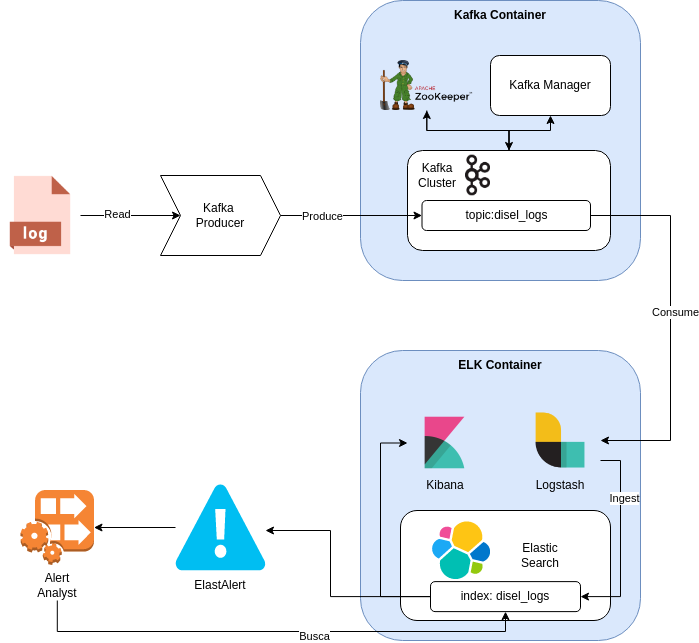
\includegraphics[width=15cm]{figuras/arquitectura.png}}
\caption{Arquitectura de la Plataforma de Gestión de Alertas}
\label{enlace1}
\end{figure}

La arquitectura estará desplegado en varios contenedores Docker. Se pueden distinguir las siguientes partes:

\begin{itemize}
\item \textbf{Producer}: como se ha comentado en el capítulo de introducción no es posible utilizar los logs de la aplicación real en el entorno de producción ya que se estaría incumpliendo la ley de protección de datos. Para ello se utilizarán logs ya registrados de los que se tiene certeza que se produjo una incidencia pero procedente de un entorno de desarrollo con datos que no contengan información sensitiva. Para reproducir el comportamiento de la aplicación se implementará un script python que se encargue de leer cada línea de log y trasladarla a kafka, de esta forma replicará el comportamiento de escribir registros a lo largo del tiempo.

\item \textbf{Kafka server}: se utilizará kafka con el fin de trasladar los datos producidos en el productos al ELK Stack. La plataforma Apache Kafka es un sistema de transmisión de datos distribuido con capacidad de escalado y tolerante a fallos. Gracias a su alto rendimiento permitirá transmitir datos en tiempo real utilizando el patrón de mensajería publish/subscribe. 

\item \textbf{ELK Stack}: conjunto de aplicaciones (Elastic Search, Logstash y Kivana). Permite recoger datos de cualquier tpo de fuente y cualquier formato para realizar búsquedas, análisis y visualización de los datos en tiempo real. En la arquitectura planteada se para la aplicación real se obtendrán los datos a partir de ficheros de logs mediante Logstash y se almacenarán en el motor de búsquedas y análisis de Elasticsearch. Además, se permite la visualización, monitorización y explotación de datos en tiempo real mediante kibana.

\item \textbf{Elastalert}: herramienta open source que se integra con ELK y permite detectar anomalías e inconsistencias en los datos de Elasticsearch y lanzar alertas. El conjunto de herramientas de \textbf{ELK (Elastic Stack)} más ElastAlert permite crear un sistema de monitorización para la extracción, almacenamiento y explotación de los datos de los procesos o sistemas a monitorizar.

\end{itemize}

\subsection{Generador de alertas}

Para detectar y emitir alertas como se comentó en el apartado anterior se utilizará ElastAlert.
ElastAlert es un componente originalmente diseñado por Yelp que es capaz de detectar anomalías, picos u otros patrones de interés. Se trata de un producto \textit{production-ready} y es un estándar de alerta conocido y aceptado dentro del ecosistema de ElasticSearch. En la documentación se especifica que "Si puede verlo en Kibana, ElastAlert puede alertarlo". ElastAlert podrá realizar distintas operaciones dependiendo que como se configuren las reglas en los ficheros de configuración. 

ElastAlert consulta periódicamente a ElasticSearch y los datos se trasladan al tipo de regla, la cual determina cuando se encuentra una coincidencia. Cuando se produce una coincidencia, se envía a una o más alertas que toman medidas en función de la coincidencia. Esto se configura mediante un conjunto de reglas, cada una de las cuales define una consulta, un tipo de regla y un conjunto de alertas. Se podrán definir tipos de regla del estilo:

\begin{itemize}
\item \textbf{Frequency}: existen una serie de X eventos en un tiempo Y. (Mismos códigos de error en un minuto)
\item \textbf{Spike}:la tasa de eventos aumenta/disminuye. (Número de peticiones por minuto sobre una operación concreta aumentan considerablemente) 
\item \textbf{Flatline}: menos de X eventos en Y tiempo. (No se realizan un mínimo de consultas a la bbdd en 1 minuto)
\item \textbf{Blacklist/Whitelist}: cuando un determinado campo coincide con una lista negra. (Se establecen unos códigos asociados a la indisponibilidad del sistema y en caso de detectarse se genera la alarma).
\item \textbf{Any}: cualquier evento que coincida con un filtro dado (Un código de error al que se le dará un trato especial).
\item \textbf{Change}: un campo tiene dos valores diferentes dentro de un tiempo (Una medida asociada a la temperatura varía drásticamente en un tiempo determinado´).

\end{itemize}

En la solución propuesta se distinguirán dos tipos de alertas principales definidas tras un estudio de los logs.

\begin{itemize}
    \item \textbf{Errores conocidos}: en la aplicación se pueden dar ciertos errores relativos a problemas de comunicaciones con otros servicios, caídas de los propios servicios así como problemas de conexión o caída con las bases de datos. Cuando se produce un error de este tipo la mayoría de operaciones van a devolver en la respuesta un código de ERROR del cual se puede obtener la información necesaria para su diagnóstico.
    
    Para este tipo de errores se generara una lista de reglas con un comportamiento similar:
    \begin{enumerate}
        \item Se detectará que se está repitiendo un código de error un número configurable de veces en un tiempo determinado.
        \item Cada regla tendrá asignado un diagnóstico y las acciones a seguir en cada caso.
        \item Se enviará un correo especificando el error detectado, el diagnóstico y los pasos a seguir al correo de notificación de incidencias.
    \end{enumerate}
    
    \item \textbf{Errores desconocidos}: por otro lado pueden darse errores desconocidos en la aplicación. Estos al contrario que los anteriores no tienen un fácil diagnóstico ni hay una serie de acciones por defecto a seguir. Se puede tratar de un gran abanico de posibilidades a la hora de buscar la causa, desde un mal tratamiento de una respuesta de un sistema o un bug que se introdujo en el código. 
    
    En este tipo de errores se buscará realizar un tratamiento de los logs aplicando Machine Learning para detectar anomalías que puedan ayudar al responsable a diagnosticar y buscar una solución. En este caso se definirá un regla, que en caso de detectar un error no definido obtenga el identificador de la transacción de la operación y haga una llamada al servicio del componente de Alert Analist con el fin de que trate los logs obtenidos.
    
\end{itemize}


\subsection{Reducción de log}

Cuando la aplicación falla con un error indeterminado se genera un log distinto al normal. Encontrar la causa del error puede ser un trabajo muy tedioso ya que involucra el estudio de los logs para encontrar la fracción del registro que se escapa de la operativa normal. Para hacer esta tarea más simple se utilizará LogReduce, el cual es un librería de código abierto que permite la generación de modelos Machine Learning entrenándolo con ejecuciones exitosas de procesos anteriores para extraer anomalías de los registros de ejecuciones fallidas.

Los logs de la aplicación se componen de un registro de los distintos servicios que permite la aplicación. Cada vez que un servicio es invocado se guardará un registro de la petición, las transformaciones realizadas sobre los datos, información referente a las casuísticas concretas y de la respuesta. El conjunto de los registros comunes en la ejecución de un servicio que finalice correctamente se conocerá como \textbf{\textit{Basenile}}.  En caso de se produzca algún tipo de error durante la ejecución del servicio se producirán excepciones que ayudarán a definir la causa del fallo.


Para eliminar los \textit{Baselines} de un log errado se podrá utilizar un algoritmo de k vecinos más próximos (\textbf{k-nearest neighbors pattern recognition algorithm k-NN}). 

Para ello, cada evento registrado en el log deberá ser convertido a un valor numérico aplicando algoritmos de Hashing Vectorizer. De esta forma se consigue mapear cada palabra y codificar cada evento en una matriz dispersa. Para mejorar este proceso se deberá aplicar una limpieza del texto quitando stop-words (palabras que no tienen significado por si solas), así como un proceso de tokenización para eliminar datos aleatorios como IPs y marcas temporales.

Una vez el modelo esté entrenado se podrá calcular la distancia de cada evento con respecto al \textit{Baseline} y mostrar aquellos resultados con un valor de distancia mayor que un umbral fijado. 

\begin{figure}[H]
\centerline{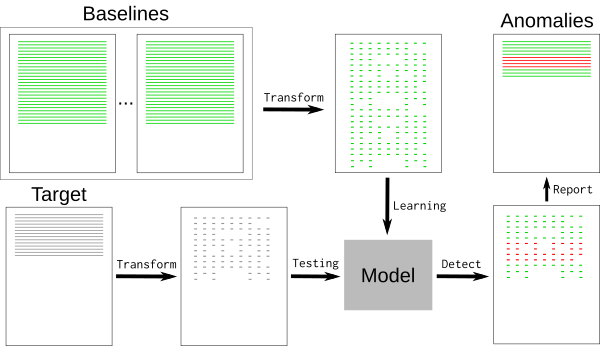
\includegraphics[width=15cm]{figuras/logreduce.png}}
\caption{Pipeline logreduce}
\label{enlace1}
\end{figure}

La librería LogReduce implementa este proceso con las ventajas de que se pueden especificar múltiples \textit{Baselines} para entrenar el modelo, así como la generación de reportes html para la mejor visualización del proceso.

El proceso de entrenamiento por tanto podrá ser cíclico de forma que en la que se vayan generando nuevos \textit{Baselines} añadirlos a la construcción del modelo. De esta forma el modelo estará preparado para cambios y evolucionará de igual manera que lo hace la aplicación. 

